\chapter{Trust graph}
\label{trust-graph}

People are still one of the most advanced technology. We can get inspired by some of the solutions that work in human societies for centuries.
Yuval Noah Harari in his book "Sapiens: A Brief History of Humankind" \cite{harari2014sapiens} states that the most important feature of human language is a rumor. Rumor let us know which person is not trustworthy without having to interact with him directly. If our best friend Bob, tells us, that Carlie is theft, we do not need to get stolen to be convinced about it. The same applies to an inverse scenario, if Bob tells us, that Carlie sells great quality products, we are now more likely to buy products from him; we are biased towards people, whom we get positive rumors. We notice that each person we know directly or indirectly gets labeled with some tags. One can be labeled as Helpful, Conscientiousness, and also Not-Trustworthy, while others can be labeled as Unhelpful, Lazy but Trustworthy. Here in this thesis, we are limiting our range of study just to the dimension of Trustworthiness.
If we have three friends Alice, Bob, Charlie. Alice and  Bob tell us that David is Trustworthy, while Charlie claims that he is not. The decision to labeling David as Trustworthy or Not-Trustworthy, requires some kind of decision evaluation algorithm.
One might assume that if there is at least one person who does not trust him, there must be something wrong with him, and will label him as Not-Trustworthy. One can use another evaluator which says, do want the majority of people do, thus if Charlie is trusted by the majority, I will trust her too. Another one can slightly generalize this evaluator and say that person is trustworthy, only if $\xi$ percentage of my friends trust him. 

At this point, it is worth introducing some conventions. When we say friend we mean a trustworthy person, in other words, a person whom we have trust relation to. Let $N$ be a set of all considered individuals. Let $F_n \subset N$ be a set of all $n$'s friends $f \in F$. Then we call 
\begin{equation}
\%(n_1, n_2) = \frac{|F_{n_1} \cap F_{n_2}|}{|F_{n_1}|}    
\end{equation}
the proportion of $n_1$ friends who are also $n_2$ friends. Let's call $\xi$ (where $0 \le \xi \leq 1$) the minimum proportion of $n$'s friends needed to make trust relation other person in a graph. $\%_n$ who needs to trust person $n$ to make me trust him. 

Going back to our example, we trust David only if majority of our friends trust him. We denote trust function as $T : N \rightarrow \{true, false\}$, $T(n) = \%_n > \xi$. 
Let's use this formula to evaluate if $David$ is a trustworthy person. Let $\xi = 0.5$. We know that Alice and Bob do trust David, while Charlie does not.
\begin{equation}
\begin{split}
T(David) &= \%_{David} > \xi \\
&= \frac{|F_n|}{|F|} > \xi \\
&= \frac{2}{3} > \frac{1}{2}
\end{split}
\end{equation}
Then $David$ is \textbf{Trustworthy}


People with low $\xi$ easily get manipulated, we call them naive.
People with high $\xi$ hardly gets convinced, we call them stubborn. 

Another generalization might be adding weights to this evaluator, let's say that Charlie is our brother, while Alice and Bob are our cousins, and we trust 3 times stronger to our brother than a cousin. Let's call $W : F \rightarrow \mathbb{N}$ the function that maps our friend to the weight of how strong we trust him. In this case weighted proportion of our friends 
\begin{equation}
\%_n = \frac{\sum\limits_{f \in F_n} W(f)}{\sum\limits_{f \in F} W(f)}
\end{equation}

When we assume weights $W(Alice) = 1, W(Bob) = 1, W(Charlie) = 3$, and $\xi = 0.5$. We can calculate weighted proportion $T(David)$ as follows:
\begin{equation}
\begin{split}
T(David) &= \%_n > \xi \\
&= \frac{1+1}{1+1+3} > \frac{1}{2} \\
&= \frac{2}{5} > \frac{1}{2}
\end{split}
\end{equation}
Then $David$ is \textbf{Not-Trustworthy}

Another thing we can observe in the context of the trust-network is time. Should we still trust our friend from elementary school if we haven't seen him for decades? We could modify the trust function to be dependent on the time, but for now, let's assume that the friendship is immortal.

Next, if we have a friend, who has a friend, we trust that person, but he will not become our friend. If someone else ask us if he should trust that person, we would say no, because we don't want to take responsibility for people who are not our friends. Therefore only the friendship relation can propagate the trust.

Having that trust network model, we can use it to generate graphs, which then can be used to simulate infection processes. 

Having that trust model, let's describe the algorithm to generate trust graphs.
We start with a $N_0$ nodes that get connected with random $E_0$ edges, in such a way that the graph is connected. Next, for each remaining node $n \in N \setminus N_0$, we connect it to one randomly selected node in current graph. When all nodes are added, for each node $n \in N$ for each node $f \in F_n$, for each node $p \in F_f \setminus F_n$ we apply $T(n, f, p)$ function, which if evaluated to true create connection between $n$ and $p$.

In Fig \ref{fig:trustgraph500} we can see the resulting trust graph for 500 nodes and $\xi = 0.5$, and its corresponding histogram in \ref{fig:trustgraph500histogram}

\begin{figure}[h!]
    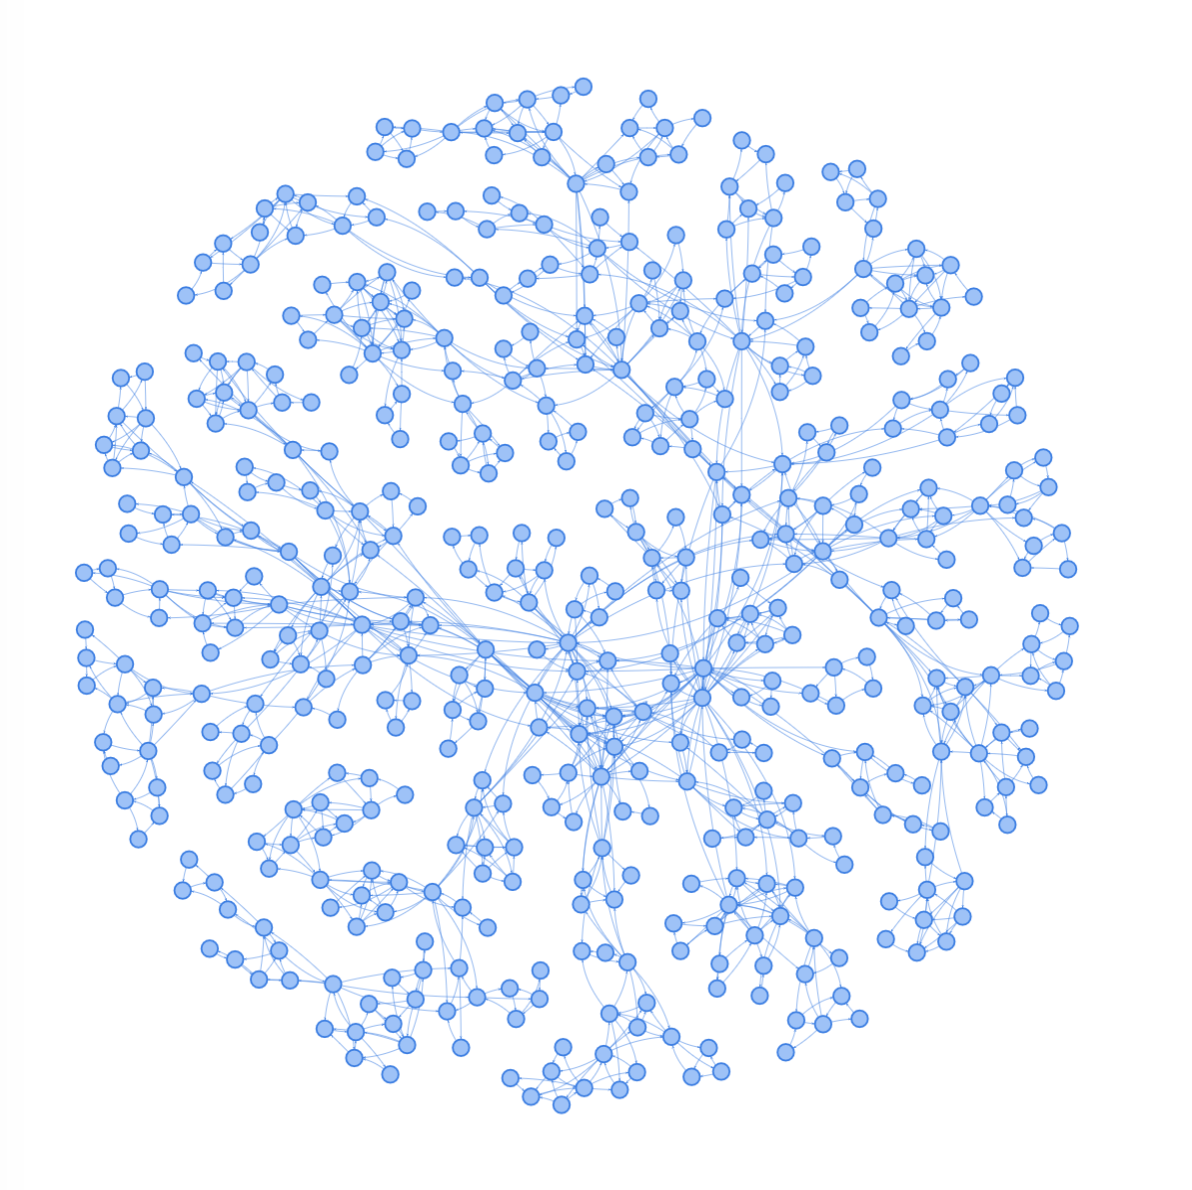
\includegraphics[width=\textwidth]{img/webOfTrust500Graph.png}
    \centering
    \caption{Trust Graph generated by Web Of Trust algorithm for $\xi=0.5$ and $n = 500$}
    \label{fig:trustgraph500}
\end{figure}

\begin{figure}[h!]
    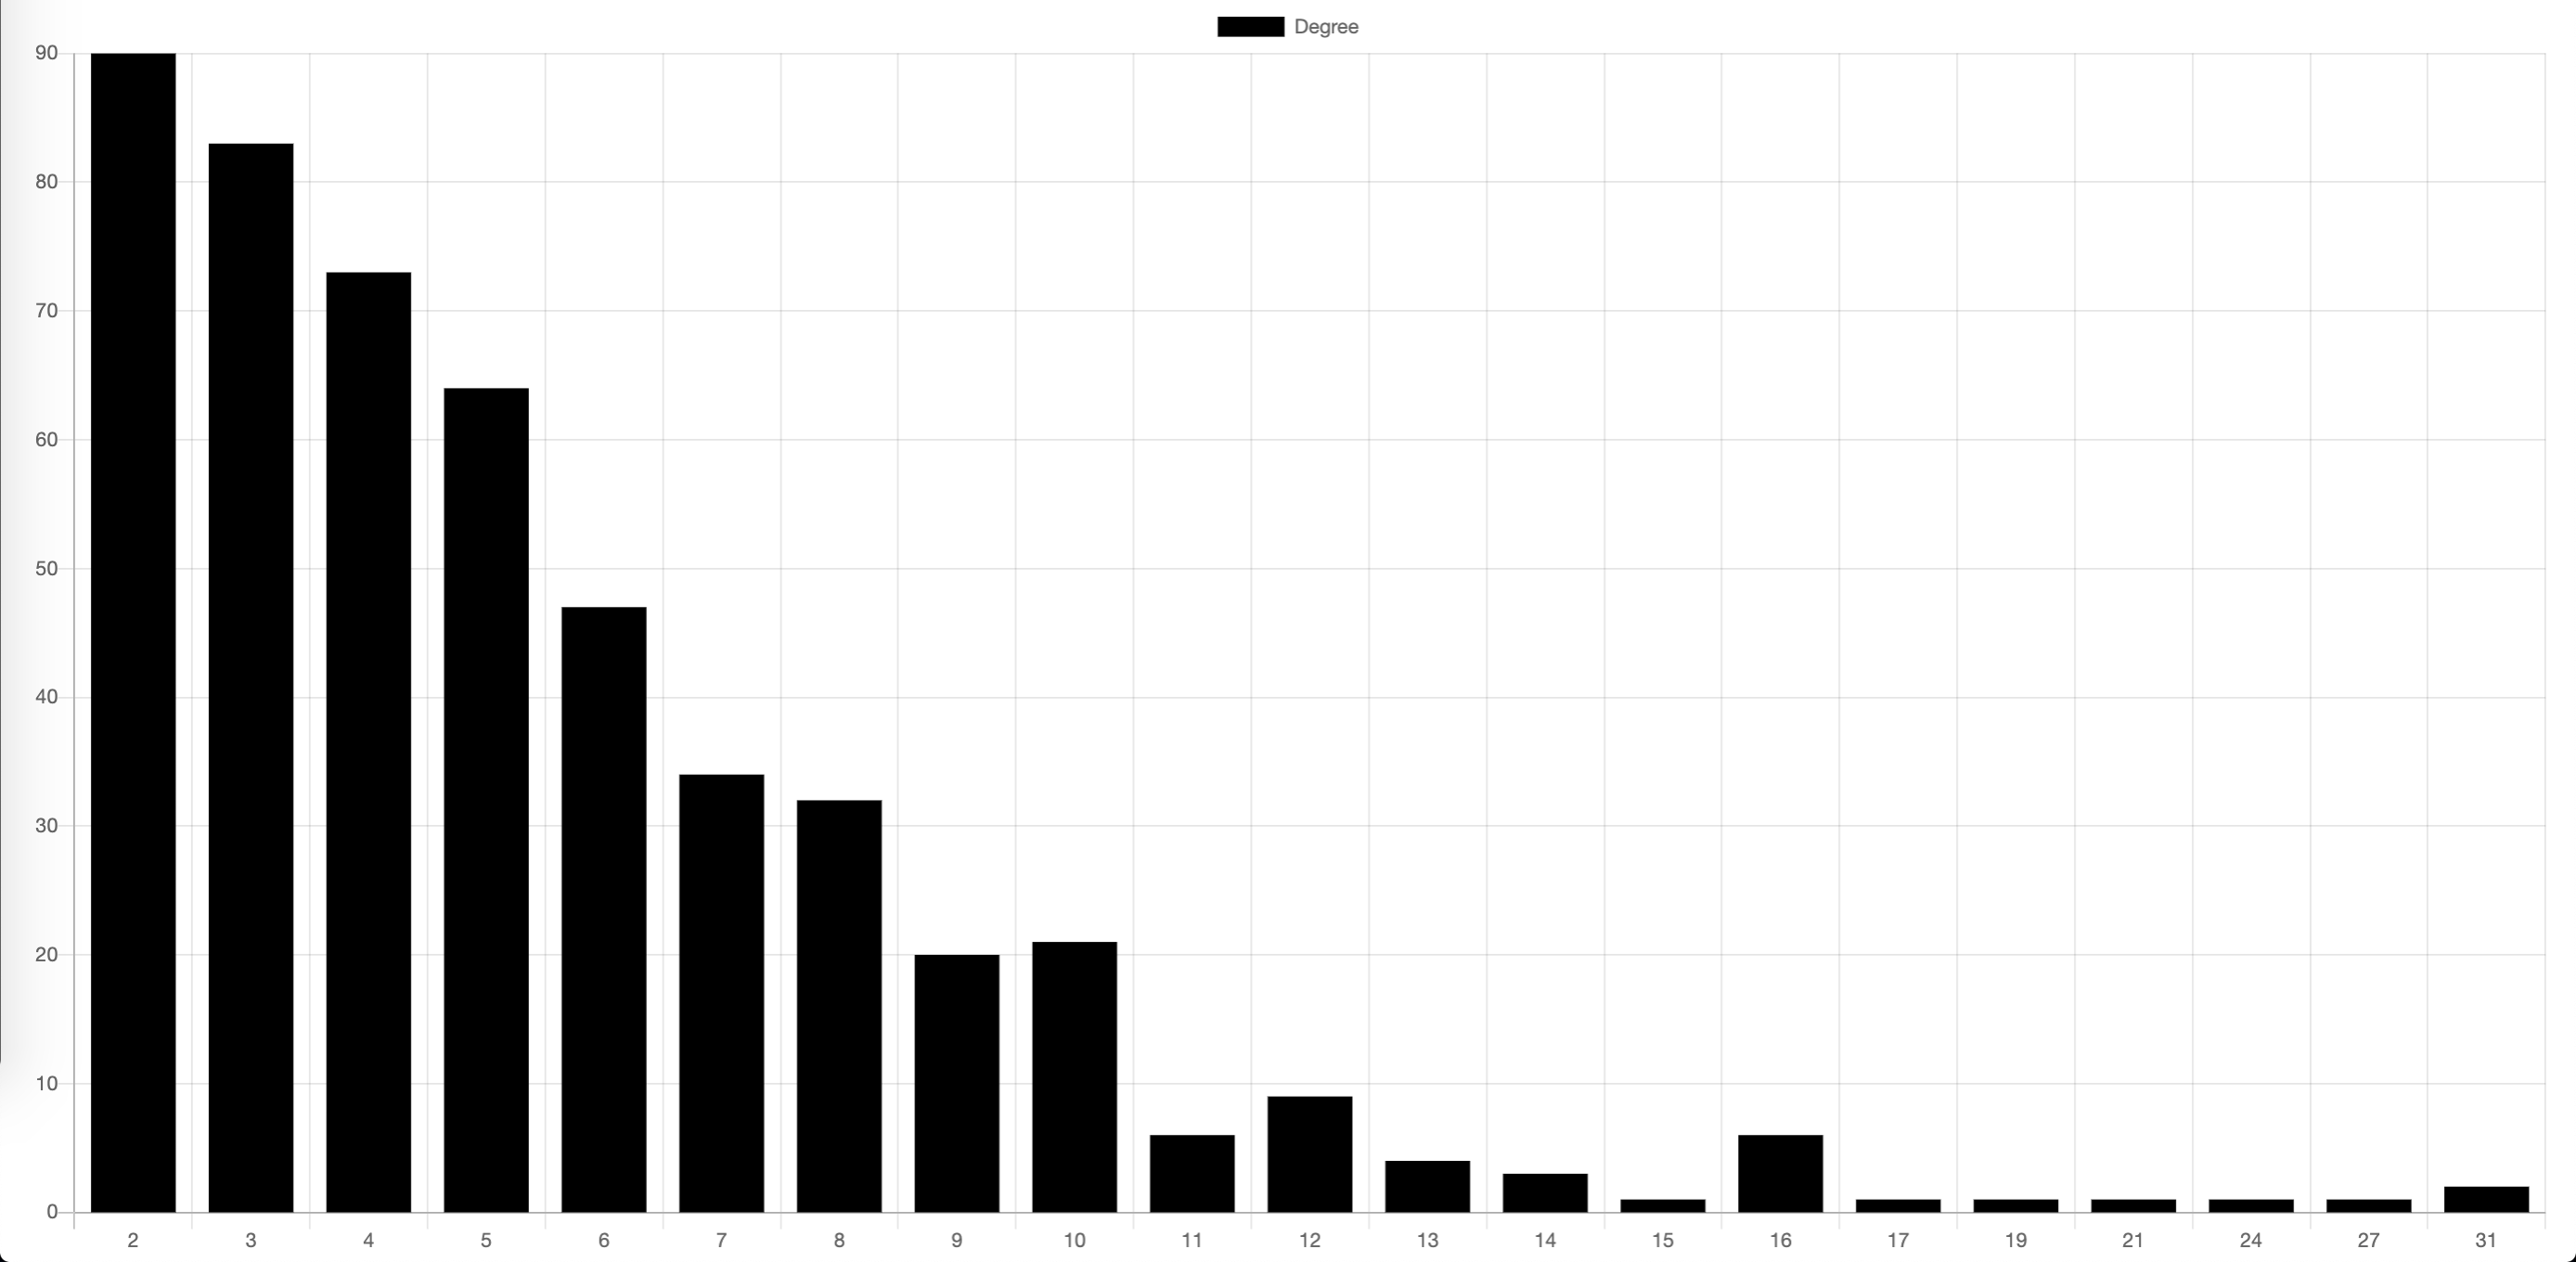
\includegraphics[width=\textwidth]{img/webOfTrust500Hist.png}
    \centering
    \caption{Degree Histogram generated by Web Of Trust algorithm for $\xi=0.5$ and $n = 500$}
    \label{fig:trustgraph500histogram}
\end{figure} 

\section{Different types of trust graph generators}

\paragraph{Probabilistic duplication}
Another trust graph generator proposed in \cite{konorski2019mitigating} base on probability duplication and can be visualized as a natural process of acquiring new colleagues at our friends' party. When we get to the party, we meet new people who with some probability become our colleagues. This algorithm works as follows: we take an initial $n_0$ nodes and $m_0$ edges and connect them randomly––creating a kernel. Then we add a new node and connect it to one random node in the current graph (your friend who invited you to his party), then with $\phi$ probability you connect to each of his friends (you acquire new friends with some of his friends), you repeat this process $n = N \textbackslash N_0$ times. 
The most important advantage of this generator is the fact that it produces scale-free graphs. Figure \ref{fig:propdup500graph} shows the graph generated by the method and Figure \ref{fig:propdup500histogram}, histogram of edge degrees.

\begin{figure}[h!]
    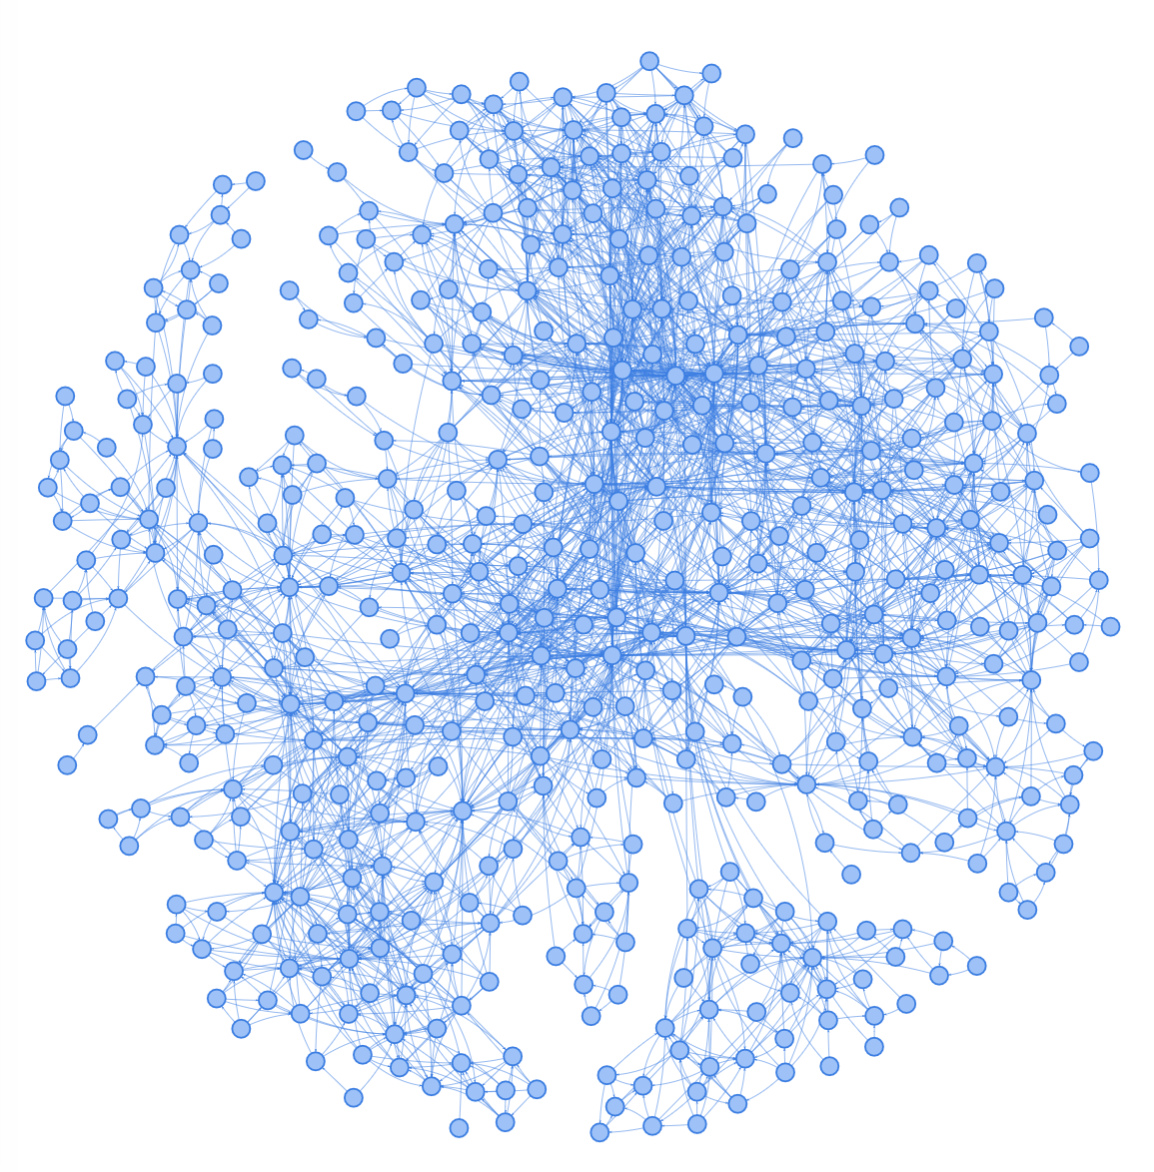
\includegraphics[width=\textwidth]{img/propDup500Graph.png}
    \centering
    \caption{Trust Graph generated by Probabilistic Duplication algorithm for $\xi=0.5$ and $n = 500$}
    \label{fig:propdup500graph}
\end{figure}

\begin{figure}[h!]
    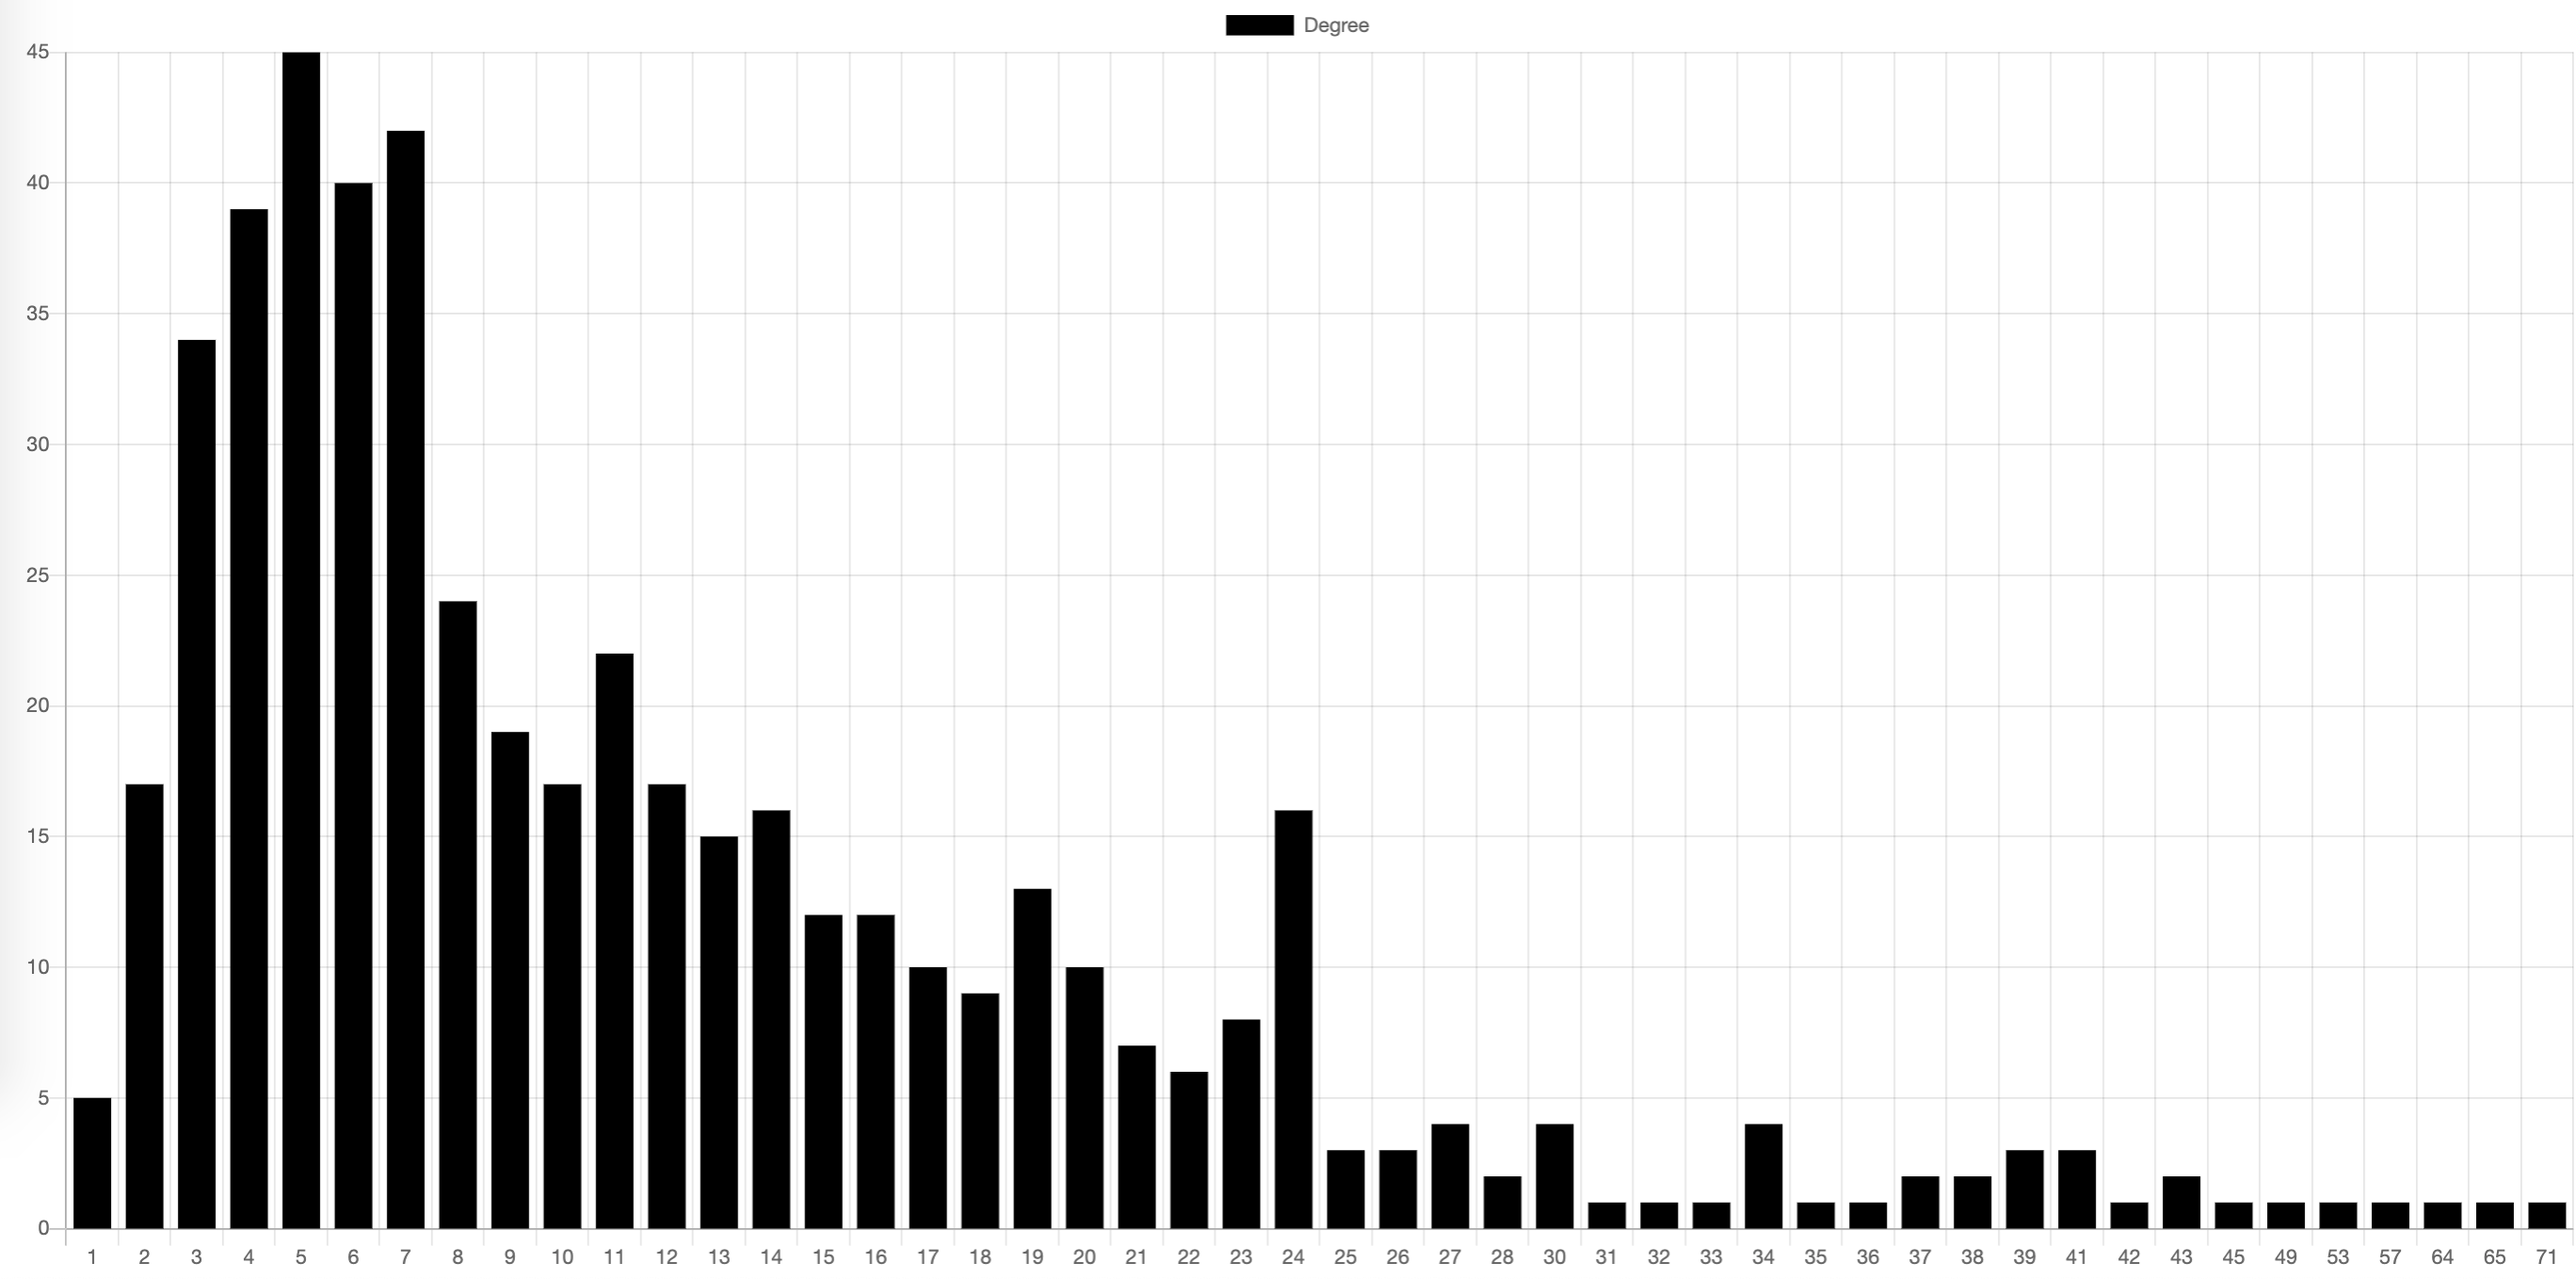
\includegraphics[width=\textwidth]{img/propDup500Hist.png}
    \centering
    \caption{Degree Histogram generated by Probabilistic Duplication algorithm for $\xi=0.5$ and $n = 500$}
    \label{fig:propdup500histogram}
\end{figure} 

\paragraph{Random generator}
Random graph generation is the simplest one. We take $n$ nodes, $m$ edges. Each edge is connected to two random nodes $n_1$, $n_2$ where $n_1 ≠ n_2$. Although random trust graphs are far from real trust graph used in reality, we will use it for comparison. Figure \ref{fig:random500graph} shows the graph generated by the method and Figure \ref{fig:random500histogram}, histogram of edge degrees.

\begin{figure}[h!]
    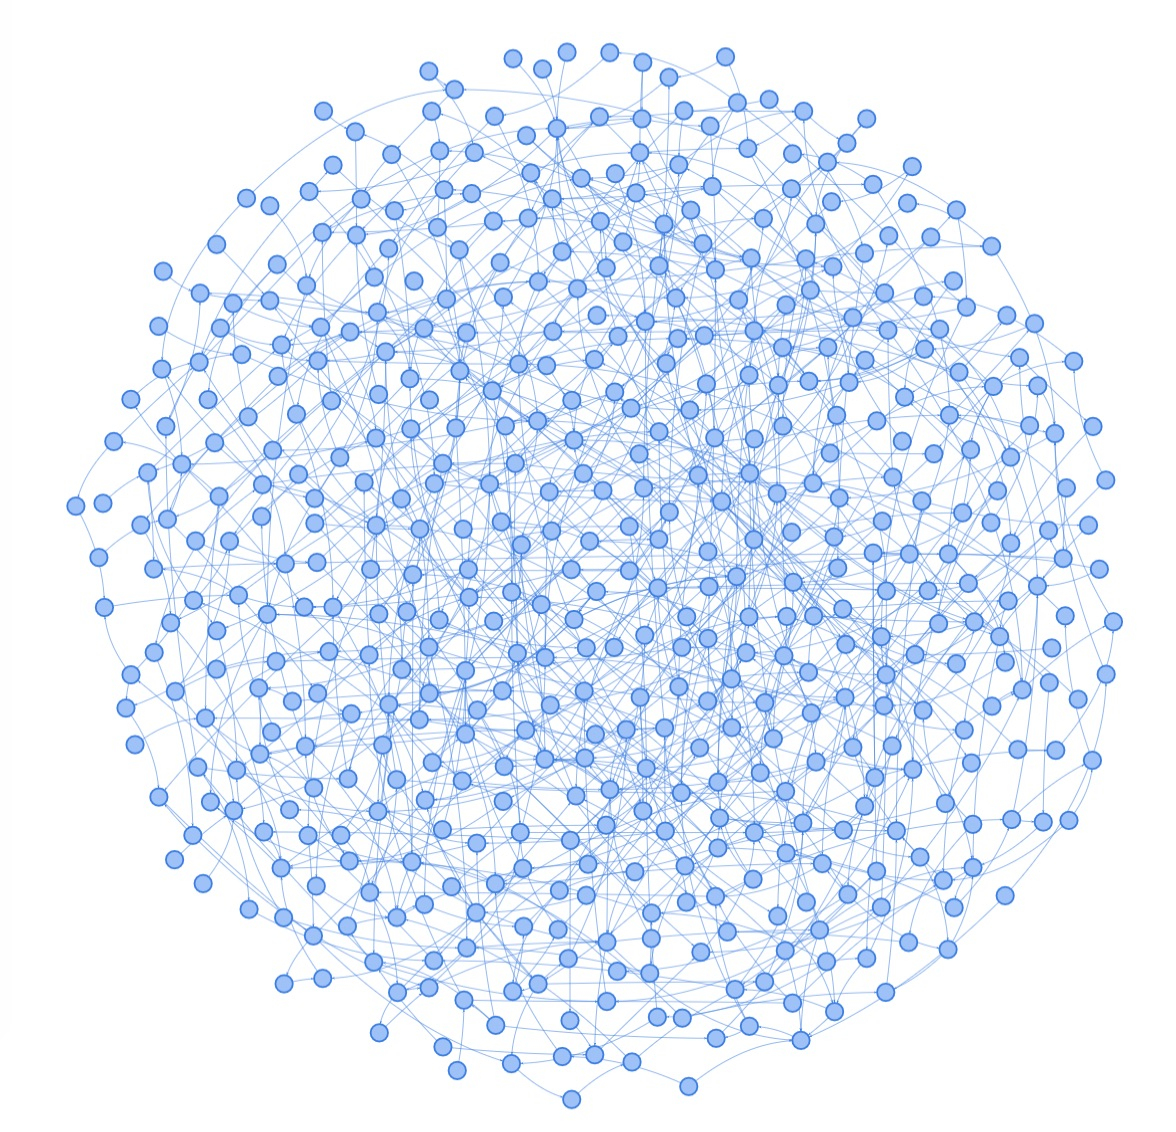
\includegraphics[width=\textwidth]{img/random500Graph.jpg}
    \centering
    \caption{Random graph generated by Random generator}
    \label{fig:random500graph}
\end{figure}

\begin{figure}[h!]
    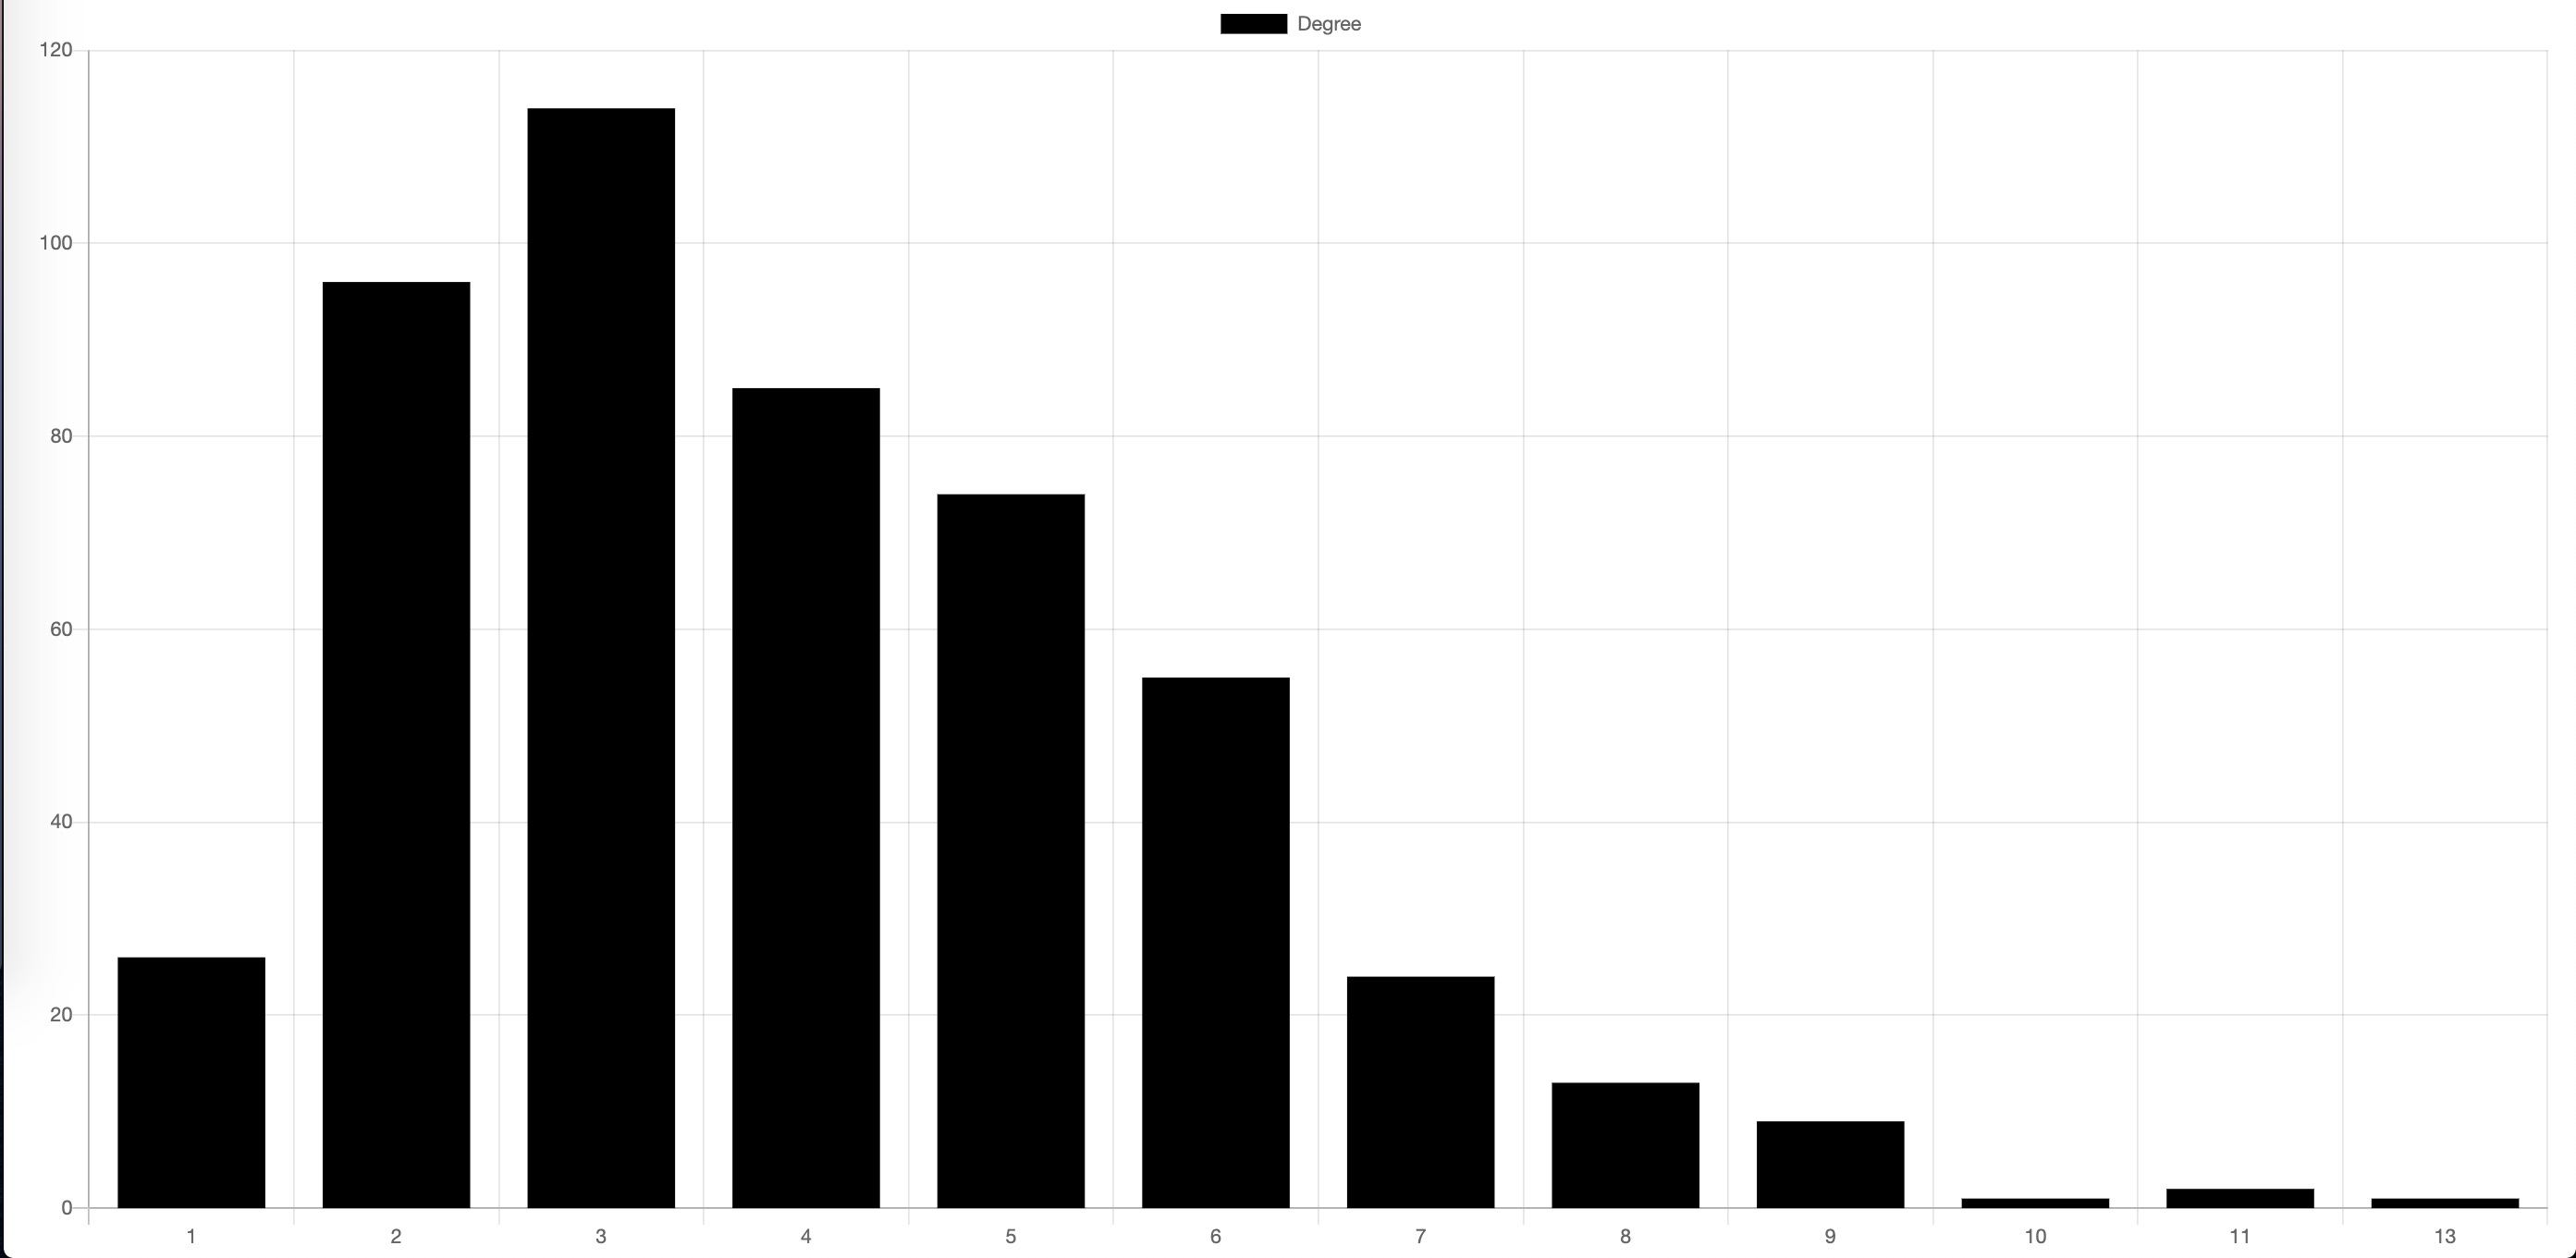
\includegraphics[width=\textwidth]{img/random500Histogram.jpg}
    \centering
    \caption{Degree Histogram generated by Random generator}
    \label{fig:random500histogram}
\end{figure} 
